\chapter{Editing images with a pre-trained GAN}
\label{chapter:magec}

%\newcommand{\mcL}{\mathcal{L}} \newcommand{\vx}{\mathbf{x}} \newcommand{\vh}{\mathbf{h}}
%\newcommand{\vy}{\mathbf{y}}
\newcommand{\tableindent}{\,\,\,\,}
\newcommand{\vt}{\mathbf{t}}
%\newcommand{\vyh}{\hat\vy}
\newcommand{\std}{$\pm\,$}
\newcommand{\clf}{\textit{clf}} \newcommand{\gray}[1]{{\color{darkgray}#1}}





% \begin{chapabstract}
%     abstract

% \end{chapabstract}
% \newpage

% \minitoc

\chapterwithfigures{\nameref*{chapter:magec}}
\chapterwithtables{\nameref*{chapter:magec}}

\ifthenelse{\boolean{skipMagec}}{\endinput}{}


\section{Introduction}

In this chapter, we aboard the question of image editing with a pre-trained deep \ac{GAN}.
For the first time, \ac{DL} models, specifically \ac{GAN}s, have achieved photorealistic synthesis \citep{karras2018progressive, karra2019stylegan, karra2020stylegan2}.
Moreover, as discussed in Chapter \ref{chapter:related}, methods have recently emerged to 
have semantic control of the generation via clever ways of manipulating the latent vector \citep{shen2020, abdal2020styleflow, harkonen2020ganspace, tewari2020stylerig, stylespace_analysis, zhuang2021enjoy, editing_style}.
 These editing methods also produce photorealistic images, contrary to concurrent image-to-image models which 
produce noticeable artifacts (albeit being more controllable) \citep{wang2018pix2pixHD, park2019gaugan}.
 In the context of image editing for the general public, latent space manipulation with the latest 
 StyleGAN2 network \citep{karra2020stylegan2}
is thus an enticing area to experiment with. 

% Generative Adversarial Networks (GANs) \cite{goodfellowgans} have made such ideas 
% possible in recent years. Recently, the celebrated StyleGAN \cite{karra2019stylegan, karra2020stylegan2} 
% has allowed unconditional generation of unparalleled quality, resolution ($1024 \times 1024$) and 
% realism. What's more, this GAN was the first of its kind to show such powerful 
% \emph{disentanglement qualities} of its latent space. For example, mixing two latent codes
%  corresponding to two images results in a coherent output image containing properties from 
%  both former images  \cite{karra2019stylegan}. This led to a surge of research into studying 
%  and manipulating this latent space, in which high-level semantic concepts  of generated images 
%  can be edited \cite{shen2020, abdal2020styleflow, harkonen2020ganspace, tewari2020stylerig, stylespace_analysis, zhuang2021enjoy, editing_style}. 
%  These editing methods produce realistic and high-quality global or local changes in the output image.

The extension to real images is natural but not trivial. A latent code first needs to be 
found such that, when inserted into the StyleGAN network, outputs the original image, a process
known as \emph{GAN inversion}.
Although inversions are able to achieve high reconstruction quality  
\citep{abdal2019image2stylegan, abdal2020}, problems arise when applying known editing methods 
onto the inverted images: the editing either does not work at all, or they produce output 
images of poor quality, presenting artifacts and blur \citep{zhu2020indomain, StyleGAN3D}. 
 We examine the reasoning behind this lack of generalization and propose a solution to this problem 
 by reframing the standard optimization framework for GAN inversion specifically in the lense of 
 editability of the reconstructed image. More precisely, we introduce a term of editability
 and i\textbf{MAG}e-lat\textbf{E}nt \textbf{C}onsistency (dubbed ``\magec'') into the global 
 loss function by using a simple yet effective procedure based on recent latent-manipulation methods.
 This allows us to explicitly incorporate 
 known editing methods into the GAN inversion optimization scheme to ensure better editability.

We validate our method with extensive qualitative and quantitative evaluation. Notably, we 
introduce a novel ``edit-consistency score'' which specifically evaluates the quality of a projection
method in terms of editability. We show that our method outperforms existing baseline methods, and
 opens the door to new possibilities of editable high-quality image inversions.

 In this chapter, we quickly go over some related work necessary for this chapter. Then, we 
 introduce our new \ac{GAN} inversion \magec framework 
which incorporates editability directly in the loss term. Then, we extensively evaluated 
our method qualitatively and 
quantitatively with standard evaluation metrics, comparing our \magec  inversion 
to existing baselines. Finally, we introduce a new 
evaluation metric, the \emph{edit consistency score} which is specifically adapted to 
evaluate both the editability and fidelity of a \ac{GAN} projection.

Our work has led to the following publication:
\begin{itemize}
  \item \fullcite{grechka_magec}
\end{itemize}



%  We introduce an i\textbf{MAG}e-lat\textbf{E}nt \textbf{C}onsistency (``\textbf{MAGEC}'') loss 
% during the inversion process. This specifically incorporates editability into the inversion
%  loss alongside with the reconstruction loss, 
% which achieves an faithful and editable reconstruction.

% In this paper, we propose a learning framework to improve editability of the projected latent 
% vector of a real image while maintaining good reconstruction. We reframe the strategy of the
%  standard optimization framework for GAN inversion. More precisely, we add a term of editability
%   and image-latent-consistency into the global loss function by using a simple yet effective 
%   procedure based on recent latent-manipulation methods. This allows us to explicitly incorporate 
%   known editing methods into the GAN inversion optimization scheme to ensure better editability. 
% We validate our method with extensive qualitative and quantitative evaluation. Notably, we 
% introduce a novel ``edit-consistency score'' which specifically evaluates the quality of a projection
%  method in terms of editability. We show that our method outperforms existing baseline methods, and
%   opens the door to new possibilities of editable high-quality image inversions.






% In this chapter, our goal was to leverage recent works on latent space manipulation 
% (see \ref{subsection:latent_space_manipulation}) to perform editing on real images. We leverage the 
% highly performant StyleGAN2 network (\ref{par:latent_space})



% We first explore real-image editing using a pre-trained \ac{GAN}. We explore the recent 
% StyleGAN (1 and 2) \citep{karra2019stylegan, karra2020stylegan2} architecutre for the specific task of real-image editing. 
% For the first time, this architecture allowed easy, fine-grained control of the generation just by cleverly modifying the values of the 
% latent vector input to the \ac{GAN}. For example, tweaking a subset of the values in this vector allows changing a specific
% characteristic of the output image, such as hair color or gender, as described in \ref{subsection:latent_space_manipulation}.
%  This type of high-level semantic editing is exactly our goal, 
% and we thus set out to apply these techniques on real images.

% In order for these methods to be applied to real images, a real image must first be inverted into the latent space of the \ac{GAN}. 
% Unfortunately, while standard inversion methods produce an accurate reconstruction of the image, they do not behave 
% well when the aforementioned latent-editing methods are applied. Indeed, the resulting image is either incorrectly 
% edited or of poor quality. We examine the reasoning behind this lack of generalization and propose a solution to this problem. Our contribution, 
% introduced in \autoref{sec:magec} introduces an i\textbf{MAG}e-lat\textbf{E}nt \textbf{C}onsistency (``\textbf{MAGEC}'') loss 
% during the inversion process. This specifically incorporates editing success into the inversion loss alongside the reconstruction loss, 
% which achieves an faithful and editable reconstruction.

% In this chapter, we will first discuss in some details the related work needed to contextualize our work.
% We go into more detail about the existing latent-space manipulation methods, introduced in \ref{subsection:latent_space_manipulation}. 
% We also discuss existing methods for GAN Inversion before detailing our own contribution to this field.



% In this paper, we propose a learning framework to improve editability of the projected 
% latent vector of a real image while maintaining good reconstruction. We reframe the strategy 
% of the standard optimization framework for GAN inversion. More precisely, we add a term of 
% editability and image-latent-consistency into the global loss function by using a simple yet 
% effective procedure based on recent latent-manipulation methods. This allows us to explicitly 
% incorporate known editing methods into the GAN inversion optimization scheme to ensure better 
% editability. 
% We validate our method with extensive qualitative and quantitative evaluation. Notably, we 
% introduce a novel ``edit-consistency score'' which specifically evaluates the quality of a 
% projection method in terms of editability. We show that our method outperforms existing baseline
%  methods, and opens the door to new possibilities of editable high-quality image inversions.





\section{Related Work}







% Editing real images in a fast and realistic way is highly lucrative for obvious reasons. 
% Users could use such a tool to visualize their personal curiosities before committing more 
% time or energy to something more permanent - How would a certain hairstyle look on me? How 
% would my house look with brick walls? Would my car look nice with different tires? Moreover, 
% a professional photographer spends around 1.5 hours of editing for a portrait image, with 
% the most costly operations being those requiring complicated semantic changes \cite{photoshop}.
%  \emph{Automatic semantic editing} is thus an application which could interest and benefit many.
 
%  Generative Adversarial Networks (GANs) \cite{goodfellowgans} have made such ideas 
%  possible in recent years. Recently, the celebrated StyleGAN \cite{karra2019stylegan, karra2020stylegan2} 
%  has allowed unconditional generation of unparalleled quality, resolution ($1024 \times 1024$) and 
%  realism. What's more, this GAN was the first of its kind to show such powerful 
%  \emph{disentanglement qualities} of its latent space. For example, mixing two latent codes
%   corresponding to two images results in a coherent output image containing properties from 
%   both former images  \cite{karra2019stylegan}. This led to a surge of research into studying 
%   and manipulating this latent space, in which high-level semantic concepts  of generated images 
%   can be edited \cite{shen2020, abdal2020styleflow, harkonen2020ganspace, tewari2020stylerig, stylespace_analysis, zhuang2021enjoy, editing_style}. 
%   These editing methods produce realistic and high-quality global or local changes in the output image.
 
%  The extension to real images is natural but not trivial. A latent code first needs to be 
%  found such that, when inserted into the \emph{StyleGAN} network, outputs the original image. 
%  Although inversions are able to achieve high reconstruction quality  
%  \cite{abdal2019image2stylegan, abdal2020}, problems arise when applying known editing methods 
%  onto the inverted images: the editing either does not work at all, or they produce output 
%  images of poor quality, presenting artifacts and blur \cite{zhu2020indomain, StyleGAN3D}. 
 
 


% In this paper, we propose a learning framework to improve editability of the projected latent vector of a real image while maintaining good reconstruction. We reframe the strategy of the standard optimization framework for GAN inversion. More precisely, we add a term of editability and image-latent-consistency into the global loss function by using a simple yet effective procedure based on recent latent-manipulation methods. This allows us to explicitly incorporate known editing methods into the GAN inversion optimization scheme to ensure better editability. 
% We validate our method with extensive qualitative and quantitative evaluation. Notably, we introduce a novel ``edit-consistency score'' which specifically evaluates the quality of a projection method in terms of editability. We show that our method outperforms existing baseline methods, and opens the door to new possibilities of editable high-quality image inversions.
% \section{Related Work}

\paragraph{Latent Space Manipulation with StyleGAN}
We briefly discussed latent space manipulation methods with \ac{GAN}s in 
Chapter \ref{subsection:image-to-image models}. We will go into a bit more detail 
on recently proposed methods, particularly detailing the methods used for evaluation 
in this chapter.

\cite{karra2019stylegan} showed in their original StyleGAN paper that 
when interpolating between two latent vectors $\z_1$ and $\z_2$ in the 
latent space, semantically "interpolated" images can be generated through
StyleGAN.

InterfaceGAN \citep{shen2020} makes use of an auxiliary classifier on faces which predicts 
the 40 CelebA \citep{celeba} attributes from a given face image. 
Then, by generating many (latent, image) pairs with the pre-trained \ac{GAN},
they obtain (latent, descriptor) training data by applying the auxiliary 
classifier. Finally, they train an independent SVM \citep{svms} for each 
binary attribute which they wish to modify with this training data. In this way,
they learn a hyperplane in the latent space which separates positive examples 
from negative examples in relation to the particular attribute, and can thus 
navigate through the latent space with the normal of this hyperplane to 
accentuate or diminish an attribute. Their method displayed convincing results 
of editing generated images, albeit attributes were entangled with one 
another (e.g. "glasses" and "old").

StyleFlow \citep{abdal2020styleflow} 
 also makes use of an auxiliary classifier and instead of 
an SVM, they use a Normalizing Flow network conditioned on the attributes
which learns a mapping between a noise vector $\z \sim \gaussian$ and the 
latent style vector of StyleGAN $\w$. Once trained, a vector $\z$ can be 
sampled with custom attributes to produce a novel $\w$ to generate 
the image wit the modified attributes. They show that their method 
effectively disentangles the latent space and produces natural edits.

GANSpace \citep{harkonen2020ganspace} 
 simply performs PCA in the latent space of the 
pretrained \ac{GAN}. Then, a manual labelling step is necessary to show 
what each of the components correspond to in the image space. This method 
has the advantage of not relying on an auxiliary classifier but is less 
controllable than the previous methods.



\paragraph{GAN Inversion} 

GAN Inversion is typically performed in one of three ways: an optimization-based 
approach which consists in optimizing a latent vector $\z$ (or a subset of the 
\ac{GAN}'s inner parameters) specifically for an input image, a learning-based 
approach, which consists in training an encoder, typically from generated training 
of the pre-trained \ac{GAN}, to predict the latent code from the input image, 
and finally, a hybrid approach, which consists in initializing the latent 
vector with the encoder's prediction before performing further instance-based 
optimization. The instance-based optimization method allows for better 
reconstruction but is time-consuming, while the learning-based method is the 
opposite.

GAN inversion has roots shortly after the appearance of \ac{GAN}s 
themselves in an effort to edit real images 
via manual drawing techniques \citep{zhu2016generative, bau2020semantic},
which used an optimization-based approach initialized with an encoding.
\cite{bau2019seeing} proposed an optimization-based inversion strategy 
which optimized the parameters of a \ac{GAN} iteratively layer by layer.
\cite{abdal2019image2stylegan} and later \cite{abdal2020} proposed 
an optimization-based method specifically to StyleGAN's style vector.

For encoder-based methods, \cite{zhu2020indomain, psp} and \cite {e4e}
recently made important progress towards encoder-based solutions, specifically 
tailored to the StyleGAN architecture, which considerably improved 
reconstruction quality compared to previous approaches. Recently, \cite{alaluf2021restyle}
proposed an encoder-based method based on iterative refinement, which consists 
in iteratively improving the encoder-based code by feeding it through the 
encoder multiple times. This improved previous solutions and only required 
$10$ forward calls, still much faster than optimization-based methods. Still,
their method loses details of the input image compared to optimization-based methods.

Because fidelity to the input image is of utmost importance when performing 
high-quality image editing, we prioritize fidelity to the input image over time 
and thus focus on an optimization-based approach.




\section{MAGEC Inversion}
\label{section:magec}



\subsection{Methodology}
 
\noindent \textbf{GAN-Inversion Framework} Given a pre-trained GAN network (generator $G$, 
discriminator $D$) and a real image $\x_{real} \in \mathbb{R}^{C\times H\times W}$ such that: $
    G : \z \in \mathbb{R}^{d} \longrightarrow \x_{gen} \in \mathbb{R}^{C\times H\times W}$.
     The GAN-Inversion goal is to find a latent code $\z_{inv} \in \mathbb{R}^{d}$ such that: 
     $G(\z_{inv}) = \x_{rec} \approx \x_{real}$.
% \asya{remove --> inutile je pense; je precise dans les datasets apres. In this work, we use the modern state-of-the-art \emph{style-based} GAN networks \cite{karra2019stylegan, karra2020stylegan2, chen2018on} in which the latent code $z \in \mathbb{R}^d$ is inserted at $n$ parts of the generator network. In this context and similarly to \cite{abdal2019image2stylegan}, we call $\mathcal{W}$ the ``native" latent space $\mathbb{R}^{d}$ and $\mathcal{W+}$ the ``extended" latent space $\mathbb{R}^{n \times d}$ which covers a greater space of possible represented images. This extended $\mathcal{W+}$ space is able to represent any real image, even out of the domain StyleGAN was trained on \cite{abdal2019image2stylegan}. This is the space we use for our work as well.\\}
 For any real $\x_{real}$ image, the instance-based optimization problem for GAN inversion is as follows:

\begin{enumerate}
    \item Initialize $\z=\z_0$. This can be a random latent vector~\citep{abdal2019image2stylegan}, 
    an "average" latent vector $\z_{avg}$~\citep{karra2019stylegan, abdal2019image2stylegan, abdal2020}, 
    or the output of a pre-trained encoder on $\x_{real}$~\citep{zhu2020indomain, zhu2016generative}.  
    
    \item Minimize over $\z$ a loss $\mathcal{L}$  between the synthesized image $G(\z)$ and the 
    original one $\x_{real}$. The basic scheme works with a $\mathcal{L}=\mathcal{L}_2$ loss for the 
    reconstruction, recently improved with some sort of perceptual loss $\mathcal{L}_{\text{percept}}$. 
    The current general framework  minimizes the following loss:
    

\begin{equation}\label{classic_inversion_with_perceptual}
    \z_{inv}  = \min_{\z}\;\;  \mathcal{L}_2(G(\z), \x_{real}) +\lambda \mathcal{L}_{\text{percept}}(G(\z), \x_{real}). \end{equation}
\end{enumerate}

Image2StyleGAN++ \citep{abdal2020}
uses two perceptual losses of an ImageNet pre-trained VGG-16 network. Recently, it has been observed 
that using the LPIPS \citep{zhanglpips2018} perceptual loss gives more robust results 
\citep{collaborative_learning, psp}, as well as adding an "ID" loss which aims at preserving 
identity \citep{psp, e4e}.


This classic GAN-inversion framework fares poorly when known editing methods are applied to the 
inverted latents (see Fig.~\ref{fig:im2stcomparison}) largely due to the fact that the latent 
vector "overfits"
to the image space, exiting the domain of the pre-trained \ac{GAN}. Our goal is to preserve accurate reconstruction, but improve editability of the 
latent vector. We solve this using a 2-part strategy. First, like recent latent-manipulation methods, 
we learn the structure of the latent space with respect to image features. Second, and unlike previous
 work, we explicitly use this learnt structure to constrain our optimization process. The method is
  summarized in Fig.~\ref{fig:training_protocol}: the novel projection strategy continues to optimize
   the image-space loss of equation \ref{classic_inversion_with_perceptual} (shown in pink), but now 
   also explicitly optimizes at the latent-level (shown in blue). With this new modeling, we can 
   explicitly add editability directly to the loss term. As we can see with in Fig.~\ref{fig:teaser},
    this allows diverse, high-quality edits of our projected latent vectors all while maintaining
     high reconstruction fidelity. 



    




% \asya{to remove maybe (or add to intro?)
% Our method is largely motivated by three observations:
% \begin{enumerate}
%     \item \textbf{Current instance-based optimization overfits to the input image and produces poor edits.} As we can see in \ref{fig:im2stcomparison}, the current state-of-the-art inverson method, Image2StyleGAN++ produces inadequate edits, presenting artefacts, blurriness, and sometimes outright absurdity. Notice how the reconstruction is practically perfect for the human eyes. This means that while the optimization problem \ref{classic_inversion_with_perceptual} successfully acheived its objective, it is inherently under-constrained. 
%     \item \textbf{The latent code of the most recent StyleGAN presents strong discriminative properties} which can be directly used for regression and classification tasks using only a single linear layer \cite{xu2021generative}.  
%     \item \textbf{An ``in-domain" latent code produces well-editable image} \cite{e4e, zhu2020indomain}. We naturally make the inverse hypothesis: a well-editable latent code must also ``in-domain''. 
% \end{enumerate}


% We thus search a way to add latent-level supervision directly in the optimization process. To enable this, we need to create a relationship between the image space and the latent space.
% }

% \subsection{Image - Latent Linkage}
\subsection{Latent-Space Supervision}

The lack of editability of previous optimization-based methods reveal that the latent vector overfits to the image space. We thus aim to supervise the latent vector directly through the latent space. Inspired by work on latent-space manipulation \note{\cite{shen2020, harkonen2020ganspace, abdal2020styleflow, tewari2020stylerig, zhuang2021enjoy}}, we also \emph{link} the latent space with the image space, but here with the explicit goal to supervise our loss. 

Consider a pre-trained deep network $F$ which inputs an image and outputs some kind of image descriptor $d$. This could be attributes, keypoints, segmentation map, etc. 

As we know from previous work \citep{xu2021generative}, the latent space of recent 
style-based generative models has high discriminative capacity. Our method aims to 
link the image descriptors to the latent vector with the simplest network possible 
so as to minimize "relearning" some part of the GAN network (and thus keep 
supervision only at the coarsest latent-level). We generate $N$ image-latent pairs and train a
 simple linear model $\linknet$ which predicts image descriptors $d$ from the latent 
 vectors $\z$.

Concretely, we train $\linknet$ using the same exact loss as the deep image descriptor network $F$ was trained with, using the predictors of $F$ as the ground-truth labels. This simple $\linknet$ will be sufficient for supervising our latent vector directly in the latent space.






% \asya{inutile je pense
% \begin{equation}\label{linknetloss}
%     \mathcal{L}_{LinkNET} = \mathcal{L}_{F}
% \end{equation}

% }

% \begin{figure}[h]
%   \centering
%     \includegraphics[width=0.6\textwidth]{images/schema.png}
%     \caption{Linking the latent space and the image space with a simple 1-layer network. We use a pre-trained deep image descriptor network $F$ which inputs images and outputs a low-dimensional description. Then, we use this network $F$ combined with a pre-trained GAN network to train the simple 1-layer $LinkNET$ model.}
%     \label{fig:im2stcomparison}
% \end{figure}







\begin{figure*}
  \centering
    \includegraphics[width=\textwidth]{images/magec/training_protocol9.png}
    \caption{Our proposed optimization framework. We initialize our $\z$ vector with $\z_0$. Then, we generate the associated image with the pre-trained generator to obtain the image-level loss. We predict the latent-level descriptor $d'$ with our pre-trained $\linknet$. We add a consistency loss of these features with the ``ground-truth'' features $d$ evaluated from our feature-extractor network $F$. We add another consistency loss over the edited descriptors (using a differentiable editor $e$) and the ``ground-truth'' edits which we obtain by modifying $d$. This MAGEC loss gives us latent-level optimization which promotes editability and an in-domain output vector.}
    \label{fig:training_protocol}
\end{figure*}


\subsection{MAGEC Loss}
Now that we have linked our image and latent space with the simple $\linknet$,
 we can define our i\textbf{MAG}e-lat\textbf{E}nt \textbf{C}onsistency ``\magec''
  loss in the following way, built from Eq.\ref{classic_inversion_with_perceptual}. 

First, we add an image-latent consistency loss over the input image and the 
latent to optimize. We obtain the ``ground-truth'' image descriptor $d$ using $F$, 
then we use our $\linknet$ to predict the image descriptor $d'$ from latent vector
 $\z$. If the latent vector correctly represents the image, it should be able to 
 predict the associated image predictors.


Second, we add an image-latent edit consistency loss. Let $e$ be a differentiable 
known editor with $i$ editing operations (for example, an editing operation can 
be \emph{add glasses}, \emph{remove wrinkles}, \emph{to woman}, etc.). We
 perform $i$ edits of the latent vector $e_i(\z)$ and edit the 
 ``ground-truth'' image descriptor $d$ accordingly to obtain
  $d_{e_i}$. Our edited latent vector should be able to predict $d_{e_i}$
   (with $\linknet$). See Fig.~\ref{fig:training_protocol} for detailed
    illustration.

The \magec loss is given as follows:

\begin{equation}\label{MAGEC}
    \mathcal{L}_{\text{MAGEC}}(\z, \x_{real}) = \underbrace{\mathcal{L}_F(\linknet(\z), d)}_{\text{image-latent consistency  %\\ between the input image and predicted latent
    }} 
    + 
    \underbrace{\frac{1}{|edits|} \sum_{i \in edits}{\mathcal{L}_F(\linknet(e_i(\z)), d_{e_i})}}_{\text{image-latent edit consistency %of the input image\\ and the corresponding edits of the predicted latent.
    }}
\end{equation}

where $d = F(\x_{real})$ and $d_{e_i}$ is the modified $d$ according to edit $i$.

Our final loss is

\begin{equation}\label{final_loss_term} \begin{split}
\mathcal{L}(\z, \x_{real}) &= \lambda_{\text{MSE}}\mathcal{L}_2(G(\z), \x_{real}) + \lambda_{\text{LPIPS}}\mathcal{L}_{\text{LPIPS}}(G(\z), \x_{real}) \\&+ \lambda_{\text{ID}}\mathcal{L}_{\text{ID}}(G(\z), \x_{real}) +  \lambda_{\text{MAGEC}}\mathcal{L}_{\text{MAGEC}}(\z, \x_{real})
\end{split} \end{equation}


\noindent where $\mathcal{L}_{\text{ID}}$ is the \emph{ID loss} introduced
 in  \cite{psp, e4e}
 based on a pre-trained ArcFace \citep{deng2018arcface} network 
 (or ResNet50 \citep{he2016resnet} network trained with MOCOv2  
 \citep{mocov2_paper} for non-face images), and $\mathcal{L}_{F}$ was the loss 
 used to train the feature extractor $F$.

As we can see in Fig.~\ref{fig:training_protocol}, our framework allows dual 
supervision, simultaneously in the image and latent spaces. We are able to
 provide latent editing directly in the loss term, which not only allows to 
 generate editable latents, but also helps to visualize which images are 
 inherently out-of-domain for the GAN in question. Moreover, this framework 
 can be incorporated into any pre-trained GAN, and allows potential further 
 constraint by combining several differentiable editing methods together.

\section{Experimental Setup}

We propose to evaluate our \magec strategy on two benchmarks typically 
used to evaluate \ac{GAN}s - Faces and Cars. We describe the experimental setup which we used 
for both of them below. We provide a detailed list of the assets 
used in our work (datasets, code, and models) in
the Appendix in~\ref{sec:MAGEC assets}.

\subsection{Experimental Setup for Face edits}

\minipar{Datasets and Evaluation editors}

We perform thorough evaluation of our method using 1000 random samples from the CelebAHQ 
\citep{karras2018progressive} dataset. We evaluate our projection on four well-known editing methods: InterfaceGAN 
 \citep{shen2020}, GANSpace \citep{harkonen2020ganspace}, StyleFlow \citep{abdal2020styleflow} and random 
 interpolation between latent vectors \citep{karra2019stylegan}.

 \minipar{Pretrained GAN Model}
 We use StyleGAN2, pre-trained on FFHQ for $1024 \times 1024$ output resolution as our
 pre-trained GAN. We use the mapped latent space $\mathcal{W}$ and similarly to 
  \citep{abdal2019image2stylegan, abdal2020, psp, zhu2020indomain, e4e}, we extend this
   space to $\mathcal{W+}$ by allowing each of the $512$-dimensional \emph{style vectors}
    to be independent of each other. 

\minipar{Training Configurations}

For the feature extractor $F$, we train an attribute-classifier
on CelebA \citep{celeba} to predict 40 binary attributes. We use a 
ResNet50 backbone \citep{he2016resnet}
and adjust the dimensions of the last fully-connected layer to 40. We finetuned 
this model by first 
training the last layer for 2 epochs with a learning rate of 0.02 and then 
finetuning 
the entire model with discriminative learning rates ranging from 0.002 to
 0.02, as described 
in \cite{howard2018universal}.
    
To train our $\linknet$ model,
we sample $50,000$ (latent, descriptor) training pairs with our pre-trained StyleGAN2. 
Note that we use the extended $\mathcal{W+}$ space for generation, meaning 
that we generate a distinct latent vector for each style block of StyleGAN2. 
We use the predicted binary labels of $F$ as our ground-truth labels for the 
$\linknet$ training.
    
For our $\linknet$ model, we use a sigmoid activation function and 
binary cross-entropy 
loss. We use 
the Adam \citep{adam} optimizer with the default parameters. We 
trained the model for $10$ epochs and evaluated on a separate validation set, 
achieving a 
$89\%$ accuracy.
    
    
Finally, we use InterfaceGAN 
\citep{shen2020} as our editor $e$ to supervise our \magec loss, 
which performs 
add/remove operations on all 40 attributes. 



\minipar{Optimization Protocol} 
We initialize $\z$ with $\z_{avg}$, by sampling 
$N = 50000$ latent vectors with StyleGAN2 and taking the average vector $\z_0 = \z_{avg}$. 
Fig.\ref{fig:avg_ffhq} shows the generated output of the average latent vector.
We use the Adam optimizer \citep{adam} with the default parameters 
($\beta_1=0.9$, $\beta_2=0.999$, $\epsilon=1e^{-08}$). We perform our training in two
 parts. First,
we use $\lambda_{\text{MAGEC}} = 3e^{-4}$, $\lambda_{\text{LPIPS}} = 5e^{-1}$, 
$\lambda_{\text{MSE}} = 1e^{-3}$ and $\lambda_{\text{ID}} = 3e^{-4}$ and perform 100 
optimization
 steps. Then, we set $\lambda_{\text{MSE}} =  \lambda_{\text{LPIPS}} = 5e^{-1}$ for another 
 100 
 optimization steps, leaving the other loss coefficients unchanged. The learning rate 
 begins at $0.07$ and is exponentially decayed with a decay factor of $0.8$ every 
 $25$ epochs. Our two-steps procedure is motivated by the fact that 
 instance-based optimization often fails at adding semantic information
  in the 
 latent vector with small optimization steps. When placing a higher weight 
 on
  $\lambda_{\text{MAGEC}}$, we direct our latent vector $\z$ to a strong point which 
  captures 
  this semantic information. Once the latent vector is within the correct 
  ``area'' of 
  the latent space, we can give more relative weight to the loss coefficients 
  related 
  to image reconstruction.



 \subsection{Experimental Setup for Car edits}

 \minipar{Datasets and Evaluation Editors}
 We evaluate  our method using random 
 images from the Stanford Cars test set \citep{stanford_cars}, not 
 used to train $F$ (detailed below). We use the GANSpace 
 \citep{harkonen2020ganspace}
  editing method to evaluate editability.

\minipar{Pretrained GAN Model}
We use StyleGAN2, pre-trained on LSUN Cars for $384 \times 512$ output resolution
as our
pre-trained GAN. We use the mapped latent space $\mathcal{W}$ and as before,
we extend this
space to $\mathcal{W+}$ by allowing each of the $512$-dimensional \emph{style vectors}
  to be independent of each other. 


\minipar{Training Configurations} 
For our feature extractor $F$, we use a pre-trained publicly available cars 
classifier \citep{pretrained_cars} which classifies the image 
into one of $196$ car models.

Since the ``average''
latent vector from the pre-trained \emph{cars} StyleGAN2 is a 
poor representation of a car
(see Fig.~\ref{fig:avg_cars}), we train an encoder 
$E$ which predicts a latent vector from an image. This was 
used to initialize the latent vector for further optimization.
We used a pre-trained ResNet50 model \citep{he2016resnet} 
as our backbone, and modified the last layers to output
a latent vector. Generated data was used for training.


We follow the same training for the $\linknet$ as before, except we use a 
softmax activation function to predict the car model, and use the 
predicted binary label from $F$ as our ground-truth label to supervise 
training. We achieve a $95\%$
accuracy on our validation set. It should be noted however, that our ground-truth 
   car predictor often classified the generated cars in the same class 
   due to high discrepancy
    between real and generated cars (generated cars generally
     don't have distinctive logos).

 Finally, we use GANSpace 
 \citep{harkonen2020ganspace} as our editor $e$ to supervise our \magec loss. 
 It's worth noting
that GANSpace does not allow edits of the car model, so our
\magec loss supervises our training in a weaker fashion than 
 before. Here, the modified ``ground-truth'' feature vector is 
 simply the image descriptor vector, since the car model should 
 not change with GANSpace edits.


\noindent \textbf{Optimization Protocol}  We initialize $\z$ with
 $\z_0 = E(\x_{real})$. Training is again effectuated in two parts.
  First, we optimize for $50$ steps using 
  $\lambda_{\text{MAGEC}}=5e^{-2}$ and $\lambda_{\text{MSE}} = \lambda_{\text{LPIPS}} = 5e^{-1}$ 
  with a learning rate of $0.08$. Then, we decrease 
  $\lambda_{\text{MAGEC}}=5e^{-8}$ with a learning rate of $0.01$ and 
  train for $50$ more steps. We use the Adam optimizer \citep{adam}
  with default parameters for  
  the training.



\subsection{Baselines}
We compare our method with Image2StyleGAN++~\citep{abdal2020}, the state-of-the-art
 optimization-based method for GAN-Inversion. This method uses the classic loss from
  Eq.~\ref{classic_inversion_with_perceptual} (using the \ac{LPIPS} \citep{zhanglpips2018} loss 
  as the perceptual loss) and first optimizes the latent vector for 1000 iterations, then
   the noise vector for 1000 iterations. We implement their method since public code is not available. 
   This loss can be seen as an ablation of the \magec 
   and ID losses from Eq.~\ref{final_loss_term}, but minimized over more iterations. We
    also perform an ablation study using our training protocol to optimize 
    Eq.~\ref{final_loss_term} but without the \magec loss. We initialize the starting 
    vector $\z_0$ for all methods 
    in the same way as us.


\begin{figure*}
  \centering
    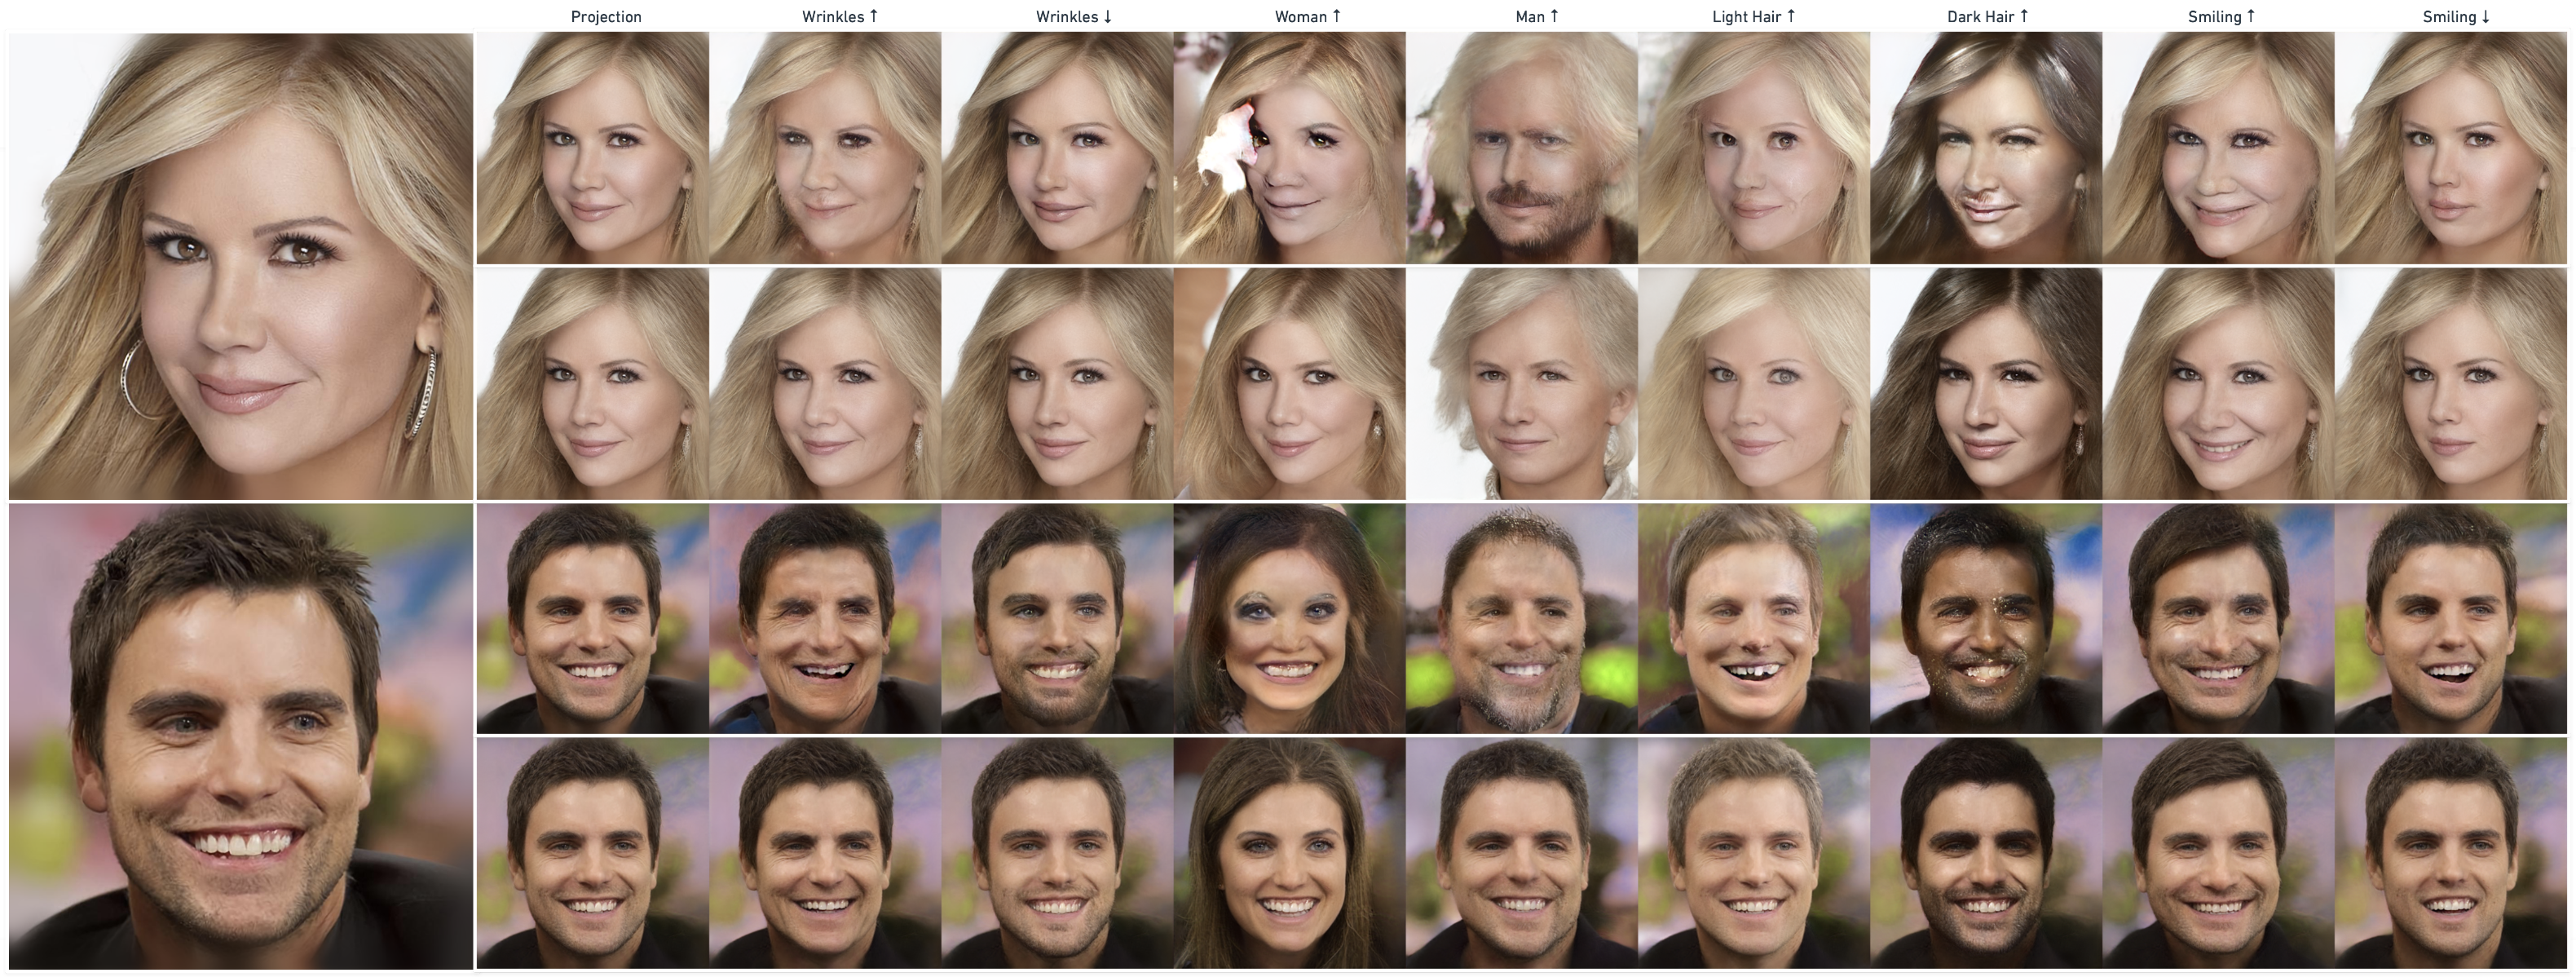
\includegraphics[width=\textwidth]{images/magec/im2st_comparison.png}
    \caption{Comparison of our method vs Im2StyleGAN++. Left: original images. Top rows: 
    Im2StyleGAN++ projection. Bottom rows: Our projection with \magec. Edits are made 
    using GANSpace. While Im2StyleGAN++'s projection is accurate, edits present strong 
    artifacts or absurdities. Our reconstructions are also accurate, but react correctly 
    to editing operations, suggesting that it follows the native distribution of StyleGAN
     more closely.}
    \label{fig:im2stcomparison}
\end{figure*}


\begin{figure*}
  \begin{subfigure}[b]{0.45\textwidth}
      \centering
      \includegraphics[width=\textwidth]{images/magec/face_average.png}
      \caption{Average latent vector from the pre-trained StyleGAN2 on FFHQ.}
      \label{fig:avg_ffhq}
  \end{subfigure}
  \hfill
  \begin{subfigure}[b]{0.45\textwidth}
      \centering
      \includegraphics[width=\textwidth]{images/magec/car_average.png}
      \caption{Average latent vector from the pre-trained StyleGAN2 on LSUN cars.}
      \label{fig:avg_cars}
  \end{subfigure}
  \caption{Average latent vectors from two different pre-trained StyleGANs}
  \label{fig:stylegan_averages}'
\end{figure*}



%\subsection{Results}

\section{Qualitative Results} 
Fig.~\ref{fig:teaser} shows our method and various 
edits applied on notorious figures. As we can see in Fig.~\ref{fig:im2stcomparison}, 
our method is visually  superior to Im2StyleGAN \citep{abdal2020} in terms of 
editing quality. While \cite{abdal2020} produces artifacts and blur during edits, our
 method produces sharp, realistic edits.

 \begin{figure*}
  \centering
    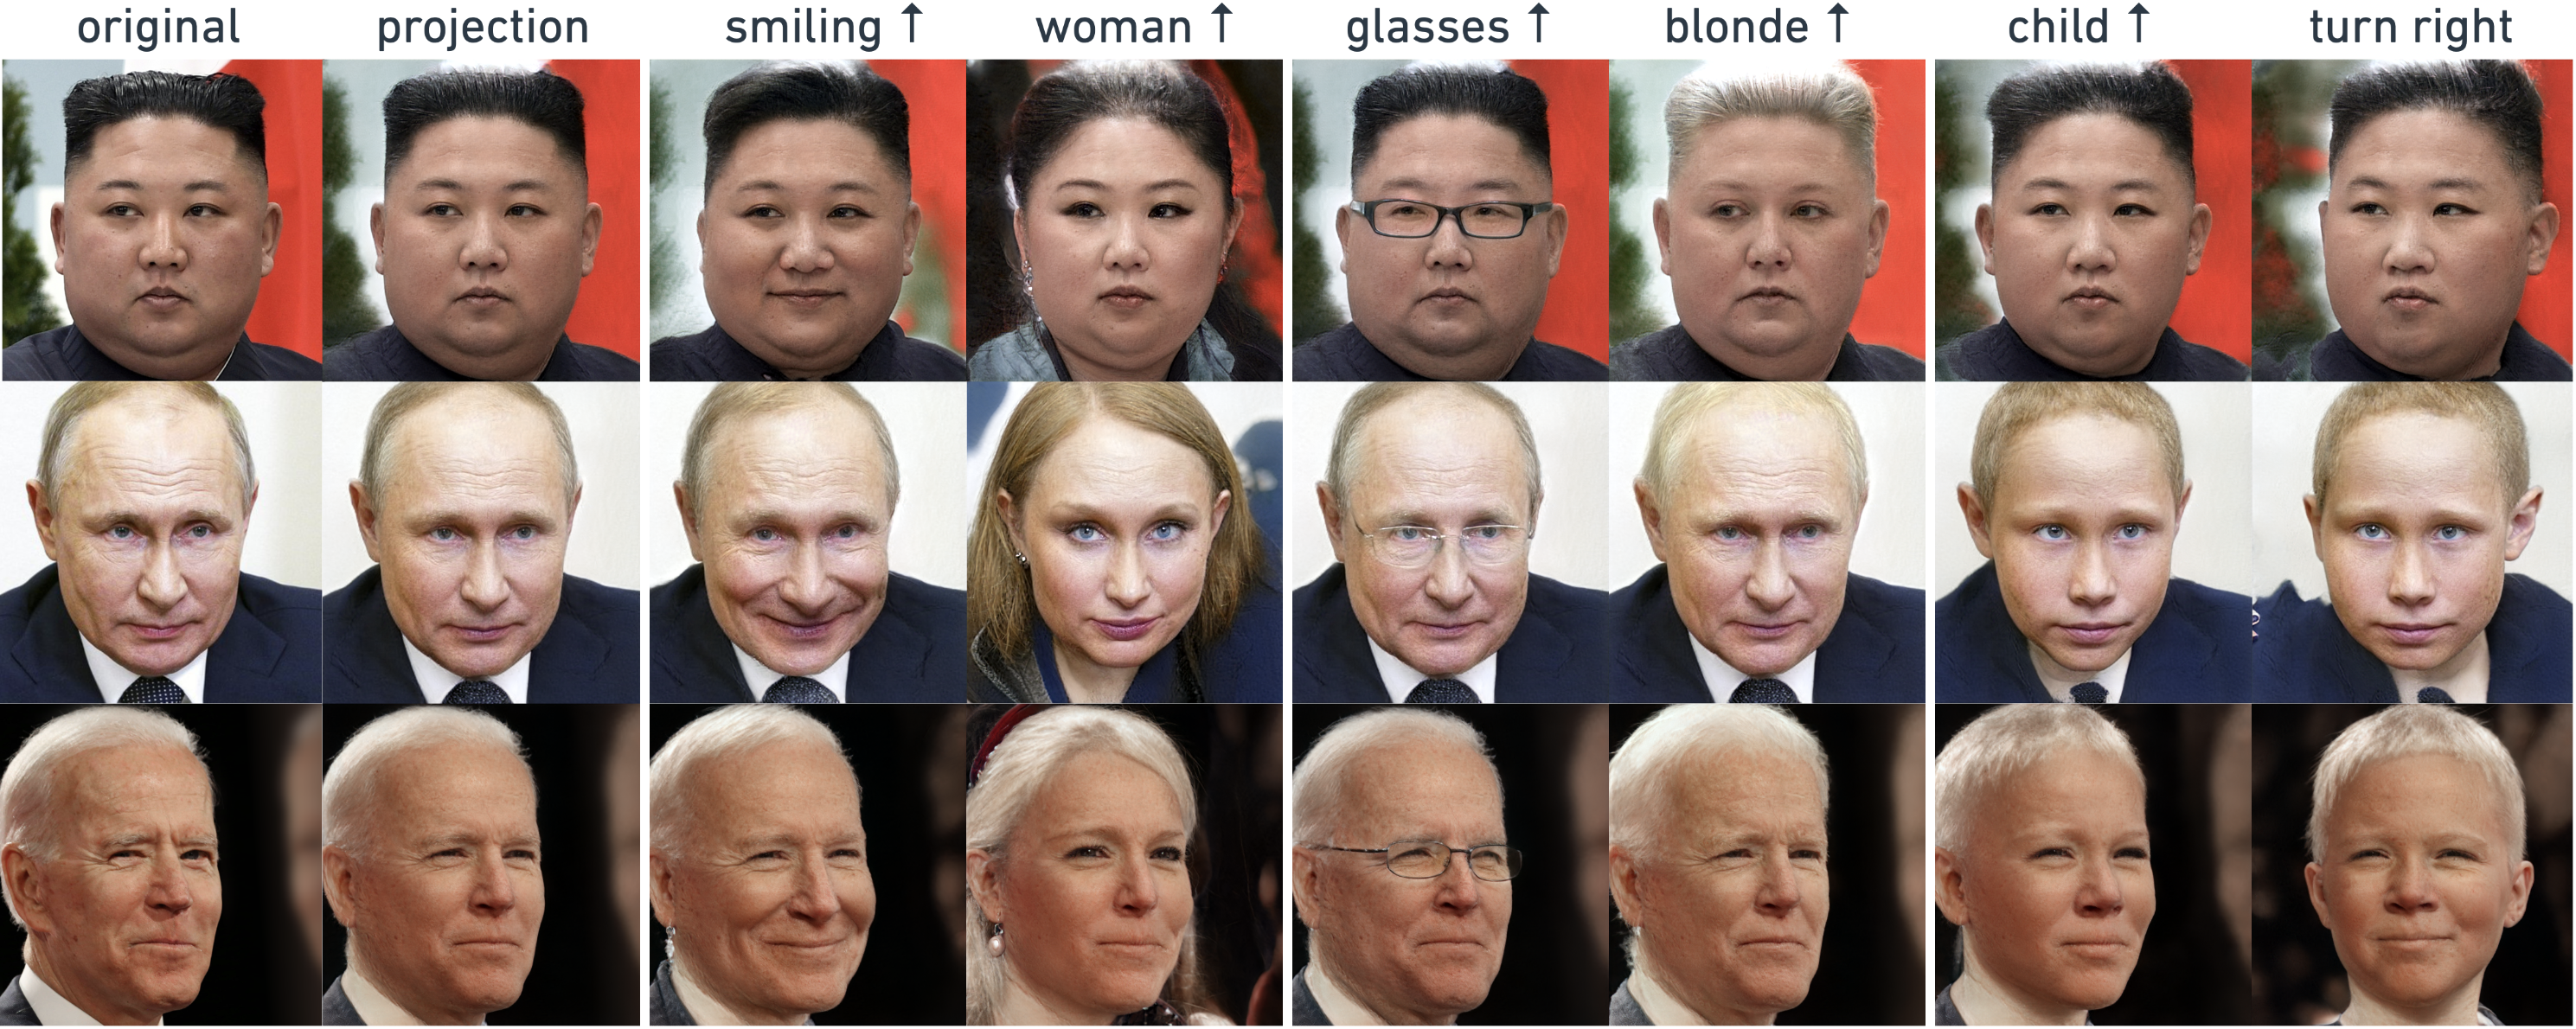
\includegraphics[width=\textwidth]{images/magec/teaser2.png}
    \caption{From left to right: original image, projection in latent space using \magec loss, various edits (GANSpace, InterfaceGAN and StyleFlow respectively). Edits are of high-quality, and conform to expectations of the various editing methods. Best viewed zoomed.}
    \label{fig:teaser}
\end{figure*}
 


In terms of assessing visual quality, human evaluation is still
 the gold standard \citep{hype, e4e}. We have thus provided 
 abundant uncurated visual results using our method and comparing
  it to Image2StyleGAN++ \citep{abdal2020} as well as to our 
  ablated method without the \magec loss. 
Fig.~\ref{fig:interfacegan_supp},~\ref{fig:styleflow_supp}, 
~\ref{fig:ganspace_sup}, and ~\ref{fig:interpol_sup} show examples with the 
respective four editing methods: InterfaceGAN \citep{shen2020}, StyleFlow
 \citep{abdal2020styleflow}, GANSpace \citep{harkonen2020ganspace}, and 
 random interpolations \citep{karra2019stylegan}. When viewing the results, 
 take extra care to notice the reconstructions (compared to the original images) as 
 well as the result of the intended edit operation (with respect to the original 
 image). Figures should ideally be viewed zoomed and in color. Note that ambiguous
  edit operations like  \emph{gender}, \emph{expression} and \emph{age} should flip
   the attribute in question (for example, \emph{age} edit means young turns to old,
    and vice versa).  The following general observations can be made:

\begin{itemize}
    \item Image2StyleGAN++ \citep{abdal2020} produces very accurate reconstructions, but edits are often of abysmal quality.
    \item Ablating the \magec loss leads to worse reconstructions.
    \item Ablating the \magec loss produces edits that are of good-quality, but often don't respect the edit intention (for example, the \emph{glasses} edit may not make any noticeable change, despite producing a high-quality image) nor fidelity to the input image.
    \item Our \magec loss gives accurate reconstructions, but also produces the intended edits that are sharper, less noisy, and of higher-quality.
\end{itemize}




Finally, we applied our method onto images of real cars. Visual results 
can also be seen in the end of this chapter in Fig.~\ref{fig:cars}. As expected, 
Image2StyleGAN++'s projection leads to distorted and inaccurate 
edits. When comparing our method to the ablated method, we can 
see that \magec helps editing and reconstruction. Notice the 
rotation operations for the first and second cars in 
Fig.~\ref{fig:cars}. The red car preserved the ``sports car'' 
look while the white car similarly preserved the \emph{Audi} 
logo .  Finally, the last rows show that we were correctly able 
to reconstruct the \emph{BMW} model as well as preserving it 
during edits.

We used a very general pre-trained classifier $F$ which was 
rather unrelated to the edits of the GANSpace editor that 
supervised our training. Moreover, our method assumes that 
StyleGAN's latent code can predict the specific car model, a 
strong assumption, especially considering that purely generated 
car images rarely have a clear logo. It is more likely that the 
latent code encodes some sort of ``shape'' which roughly predicts
 the car model with $\linknet$. Despite these limits, we can see that
  adding this simple \magec loss using an arbitrary auxiliary 
  classifier does indeed improve editing and reconstruction 
  capacity for many cases, giving high promise to the capacity and
   flexibility of our method.




   \begin{figure*}
    \centering
      \includegraphics[width=0.93\textwidth]{images/magec/interfacegan_large.jpeg}
      \caption{InterfaceGAN \citep{shen2020} edits using various inversion methods.  Our method gives the intended edits with high-quality results. Best viewed zoomed and in color.}
      \label{fig:interfacegan_supp}
  \end{figure*}
  
  \begin{figure*}
    \centering
      \includegraphics[width=\textwidth]{images/magec/styleflow_large.jpeg}
      \caption{StyleFlow \citep{abdal2020styleflow} edits using various inversion methods. Remark that here, the edits should be \textbf{cumulative}. Our \magec loss helps to produce accurate reconstructions as well as the intended edits with high-quality results.}
      \label{fig:styleflow_supp}
  \end{figure*}
  
  \begin{figure*}
    \centering
      \includegraphics[width=\textwidth]{images/magec/ganspace_large.jpeg}
      \caption{GANSpace \citep{harkonen2020ganspace} edits using various inversion methods. Image2StyleGAN++'s inversion method produces accurate reconstructions, but distorted and low-quality edits. Using our \magec loss greatly helps with reconstruction, but also helps to produce the intended change (notice \emph{male} / \emph{female} edits in particular). Best viewed zoomed and in color.}
      \label{fig:ganspace_sup}
  \end{figure*}
  
  \begin{figure*}
    \centering
      \includegraphics[width=\textwidth]{images/magec/interpol_large.jpeg}
      \caption{Interpolations \citep{karra2019stylegan} using various inversions. Take extra notice of the reconstructions, where our \magec loss clearly helps. In the first edit, only our edit gives a beard which clearly progressively disappears (rather than increasing then decreasing), suggesting stronger semantic information in the inverted latent. In the last case, notice the gradual background changes in the third set with our method, compared to the harsher change of Im2StyleGAN++'s edit.  Best viewed zoomed and in color.}
      \label{fig:interpol_sup}
  \end{figure*}
  
  \begin{figure*}
    \centering
      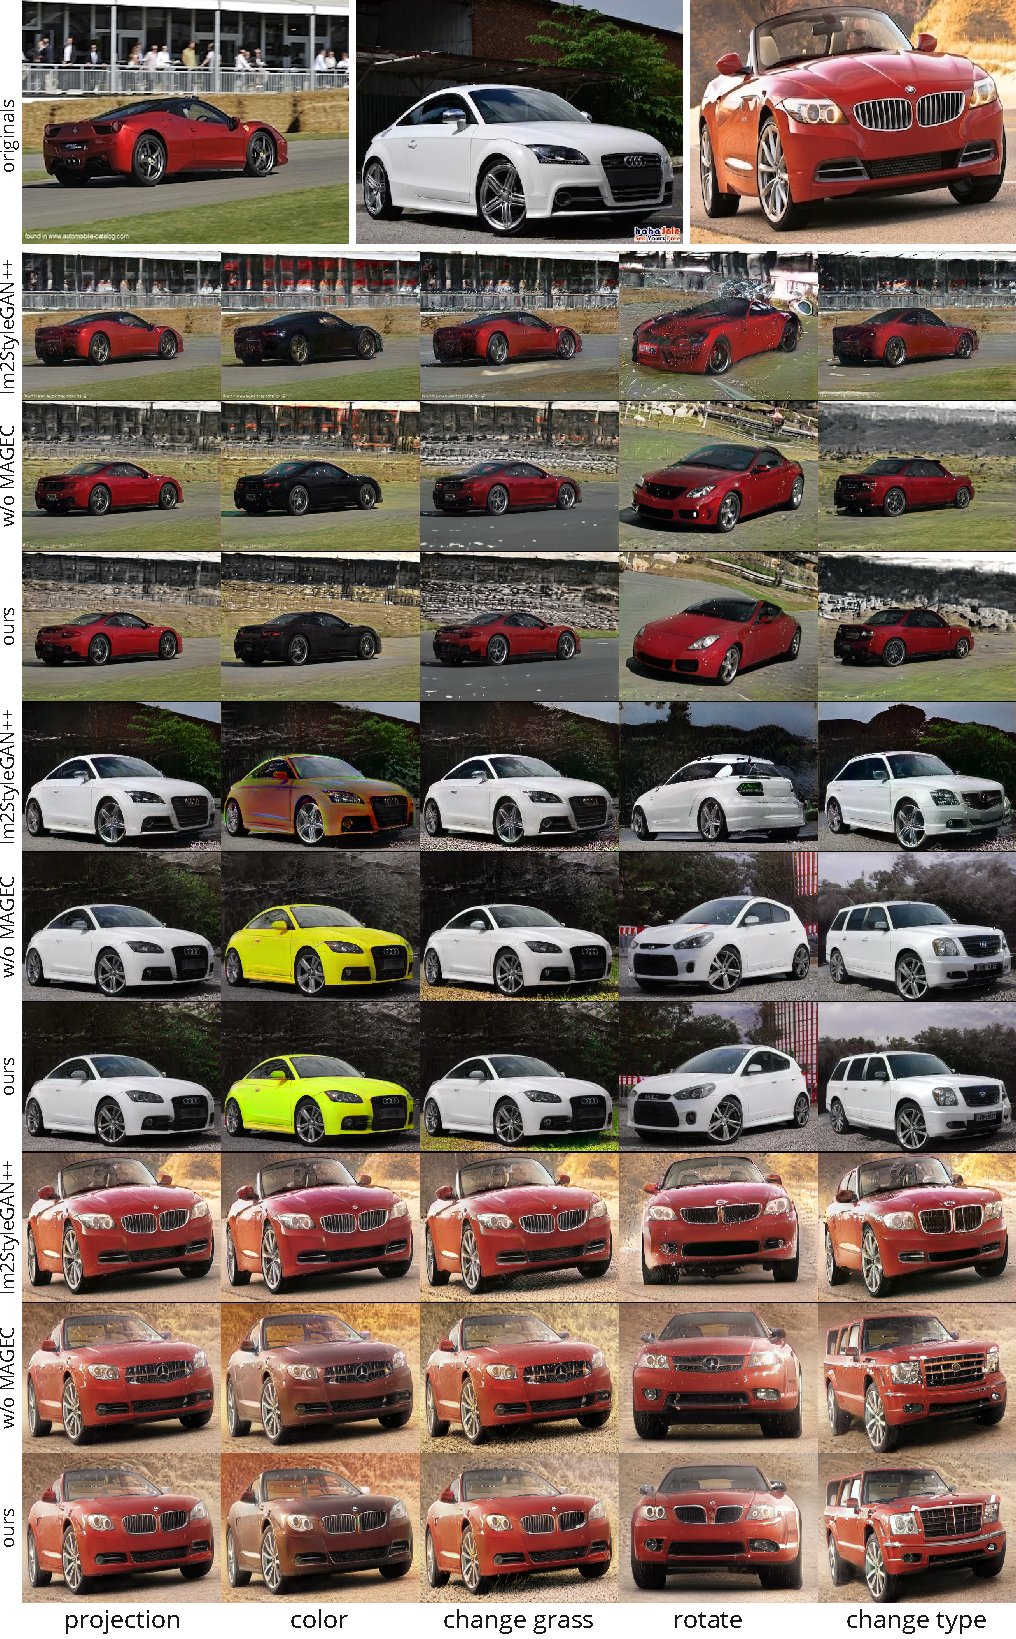
\includegraphics[width=0.835\textwidth ]{images/magec/cars_super_large.pdf}
      \caption{GANSpace \citep{harkonen2020ganspace} edits with various inversions. Image2StyleGAN++'s method produces good reconstructions but distorted edits. Our method helps in preserving the car model during reconstruction and edits. Remark the top red car when rotated: our method preserves the \emph{sports car} style. Remark that the \emph{Audi} logo of the white car is also conserved when rotating. Finally, the bottom red car reveals that our method consistently maintains the correct car model (\emph{BMW}) during reconstruction and edits. Best viewed zoomed and in color.}
      \label{fig:cars}
  \end{figure*}

\section{Quantitative Evaluation} 

\subsection{Reconstruction and Editability}

Tab.~\ref{tab:reconstruction_results} shows the various
 metrics for reconstruction. Notice that adding our \magec loss in Eq.~\ref{final_loss_term} leads a better reconstruction. Even when allowing 50\% more iterations, our method still performs on par in terms of reconstruction. The \magec loss could thus be seen as a prior which speeds up optimization. As expected, \cite{abdal2020} performs excellent reconstruction, given the time (over 4 minutes) and the under-constrained loss function.

% 11041917

\begin{table}[]
\begin{tabular}{|l|l|l|l|l|}
\hline
{  }                             & {  MSE $\downarrow$}    & {  LPIPS $\downarrow$} & {  Nb opt. steps $\downarrow$} & {  Time (s) $\downarrow$} \\ \hline
{  Full Method}                  & {  0.0040} & {  0.053} & {  200}           & {  34.6}     \\ \hline
{  w/o \magec}                    & {  0.0094} & {  0.062} & {  200}           & {  29.7}     \\ \hline
{  w/o \magec + extra opt. steps} & {  0.0078} & {  0.050} & {  300}           & {  44.5}     \\ \hline
{  Im2StyleGAN++}                  & {  0.0012} & {  0.018} & {  2000}          & {  242.2}    \\ \hline
\end{tabular}\caption{Reconstruction evaluation of projection, showing averages per image. We should note that the time of our method directly depends on the number of attributes we add to our \magec loss (Eq.~\ref{MAGEC}). Here, adding editing constraints for 40 attributes leads to a cost of about 5 seconds per image.}\label{tab:reconstruction_results}
\end{table}


We perform random edits on the 1000 images to obtain 20000 edited images per projection 
method. The semantic editability of the inverted latent vector is of utmost importance 
when performing GAN Inversion, but there is no standard metric for measuring this. We 
first evaluate using common metrics before introducing our novel ``editability score''.

We aim to evaluate the realism and ``coherence'' of a given edit. The \ac{FID} score 
\citep{fidscore} is not adapted to measure the quality of the edits, firstly because the 
original sample size (1000 original images) is well-below the recommended 50,000 needed 
for an accurate \ac{FID} score, and secondly because our edits inherently lack diversity 
(edits of the same image resemble each other).
Instead, we use the \emph{realism score} \citep{precision_recall}, which evaluates an 
image instead of a distribution. This is a nearest-neighbor based method 
(higher is better) in which the \emph{realism threshold} is set to $1$ (a score above 
$1$ is a realistic image). 

To measure the ``coherence'' of an edit, we calculate a simple ``improved-target'' score
 $t$ to measure the net difference of the predicted attribute probability before and 
 after the attribute-targeted edit by using a pre-trained attribute classifier. We use 
 our trained attribute classifier $F$ to predict this score. A higher
  value means that the attribute prediction increased after applying the editing method,
   meaning it reacted accordingly. Note that $t \in [0, 1]$. Remark that this metric is 
   only applicable to the editors which make attribute-specific edits (InterfaceGAN 
   and StyleFlow).

For reliable interpretation of these metrics, we performed a paired Student's t-test on 
our method and a competing method, as the edit operations were the same for all projected
 images. Our results are summarized in Tab.~\ref{tab:standard_metrics}. As we can see, 
 our method performs well on these metrics, always among the best in terms of realism or 
 ``coherence". However, these results are not entirely conclusive, and we investigate a 
 better metric in order to evaluate the editability of a given inversion.

% \begin{table}[]
% \begin{tabular}{lcccccc}
% \hline
% \multicolumn{1}{|l|}{}               & \multicolumn{2}{c|}{InterfaceGAN}                                                      & \multicolumn{2}{c|}{StyleFlow}                                                         & \multicolumn{1}{c|}{GANSpace}         & \multicolumn{1}{c|}{Interpolations} \\ \hline
% \multicolumn{1}{|l|}{}               & \multicolumn{1}{c|}{\textit{realism $\uparrow$}} & \multicolumn{1}{c|}{\textit{t $\uparrow$}} & \multicolumn{1}{c|}{\textit{realism $\uparrow$}} & \multicolumn{1}{l|}{\textit{t $\uparrow$}} & \multicolumn{1}{c|}{\textit{realism $\uparrow$}} & \multicolumn{1}{c|}{\textit{realism $\uparrow$}}      \\ \hline
% \multicolumn{1}{|l|}{Im2StyleGAN++ \cite{abdal2020}} & \multicolumn{1}{c|}{0.99}          & \multicolumn{1}{c|}{0.08}                    & \multicolumn{1}{c|}{0.98}          & \multicolumn{1}{c|}{0.19}                   & \multicolumn{1}{c|}{0.97}          & \multicolumn{1}{c|}{0.99}               \\ \hline
% \multicolumn{1}{|l|}{w/o MAGEC}      & \multicolumn{1}{c|}{\textbf{1.01}}          & \multicolumn{1}{c|}{0.09}                    & \multicolumn{1}{c|}{\textbf{0.99}} & \multicolumn{1}{c|}{0.15}                   & \multicolumn{1}{c|}{\textbf{0.99}} & \multicolumn{1}{c|}{0.99}               \\ \hline
% \multicolumn{1}{|l|}{Full Method}    & \multicolumn{1}{c|}{\textbf{1.01}} & \multicolumn{1}{c|}{\textbf{0.10}}           & \multicolumn{1}{c|}{\textbf{0.99}}          & \multicolumn{1}{c|}{\textbf{0.20}}          & \multicolumn{1}{c|}{\textbf{0.99}} & \multicolumn{1}{c|}{\textbf{1.05}}      \\ \hline
%                                      & \multicolumn{1}{l}{}                  & \multicolumn{1}{l}{}                           & \multicolumn{1}{l}{}                  & \multicolumn{1}{l}{}                           & \multicolumn{1}{l}{}                  & \multicolumn{1}{l}{}                      
% \end{tabular}\caption{Evaluation of random edits with \emph{realism scores} and an ``improved targets'' score by using a pre-trained classifier. While these results along are not conclusive, our method still responds well to edits and produce realistic edits according to the \emph{realism score}.}\label{tab:standard_metrics}
% \end{table}

% \usepackage{arydshln}


\begin{table}
\centering
\begin{tabular}{|l|c|c|c|c|c|c|}
\hline
               & \multicolumn{2}{c|}{ InterfaceGAN} & \multicolumn{2}{c|}{ StyleFlow} &  GANSpace &  Interpolations \\ \hline
               &  \textit{realism}      &  \textit{t}         &  \textit{realism}    &  \textit{t}        &  \textit{realism}  &  \textit{realism}        \\ \hline
 Im2StyleGAN++  &  0.973                 &  0.096     &  0.929               &  \textbf{0.211}    &  0.960             &  1.00           \\ \hline
 w/o MAGEC loss &  \textbf{0.994}        &  0.097              &  \textbf{0.976}      &  0.148             &  \textbf{0.985}    &  \textbf{1.03}                    \\ \hline
 Full Method    &  \textbf{0.998}        &  \textbf{0.122}     &  \textbf{0.982}      &  \textbf{0.202}    &  \textbf{0.984}    &  \textbf{1.04}           \\ \hline
\end{tabular}\caption{ \emph{Realism scores} and ``improved target'' scores of random image edits. For reliable interpretation, we perform a paired Student's t-test between our method's metrics and the competing method. The bold values are in line with this significance (\emph{p}-value $< 0.05$). Our method consistently produces realistic and coherent images for the task at hand.}\label{tab:standard_metrics}
\end{table}




\subsection{Edit-Consistency Score}

The standard metrics at evaluating image quality are poorly adapted to evaluating a 
projection. Firstly, as we saw in the previous section, reconstruction and editability 
metrics are independent, which makes it difficult to choose a good trade-off without an 
ad hoc solution. Moreover, the standard image quality metrics presented in Tab. \ref{tab:standard_metrics}
have no way of evaluating whether or the edited image is coherent with regards to the input image. 
We aim to address both of these weaknesses with a custom metric, the \emph{edit-consistency score}.
 
 We first use 
our projection method $p$ to obtain vector $\z$ from $\x_{real}$. Then, we use a known 
editing method $e$ to edit the vector with respect to a certain attribute, giving us
 $\x_{edit}$. Then, we re-project it into the latent space to obtain $\z'_{edit}$. Finally,
  we apply the inverse editing method onto $\z'_{edit}$ to obtain a cyclic image 
  $\x_{cyc}$, which should ideally match the initial projection.
  Fig.~\ref{fig:ecs_intuition} shows an overview of how we calculate this score.
  
  We define the 
  edit-consistency loss as follows:

\begin{equation}
    ecs(p, \x_{real}) = \frac{2 \times \mathcal{L}_{\text{LPIPS}}(p(\x_{real}), \x_{cyc})}{\mathcal{L}_{\text{LPIPS}}(p(\x_{real}), \x_{edit}) + \mathcal{L}_{\text{LPIPS}}(\x_{edit}, \x_{cyc})}
\end{equation}


\noindent The intuition is that the cyclic image should resemble the projected image, but
 images should also react accordingly to editing methods.
Remark that a ``perfect'' $ecs$ score is $0$. An $ecs$ of $1$ can be seen as a 
``quality'' threshold, since $ecs > 1$ means that the distance
 $\mathcal{L}_{LPIPS}(p(\x_{real}), \x_{cyc})$ is larger than one of the two edit
  operations.
 See Fig.~\ref{fig:ecs_examples} for examples of varying $ecs$ scores. We can now define 
 the edit-consistency score of a projection :
  \begin{equation} ECS(p) = \frac{1}{|X|}\sum_{\x_{real} \in X}{ecs(p, \x_{real})}. \end{equation}


\begin{table}
    \centering
\begin{tabular}{|l|l|l|l|l|}
\hline
              & \multicolumn{2}{c|}{ InterfaceGAN}             & \multicolumn{2}{c|}{ GANSpace}                          \\ \hline
              &   \textit{Male} $\downarrow$ &   \textit{Smile} $\downarrow$ &   \textit{Male} $\downarrow$ &   \textit{Smile} $\downarrow$ \\ \hline
  Im2StyleGAN++ &   0.97     &   1.00               &   1.07              &   0.98               \\ \hline
  w/o \magec     &   1.01             &   0.95                       &   1.06                      &   0.90                       \\ \hline
  Full Method   &   \textbf{0.84}             &   \textbf{0.87}                       &   \textbf{0.95}                      &   \textbf{0.79}                       \\ \hline
\end{tabular}
\caption{$ECS$ evaluation. Our \magec loss significantly improves $ECS$ for all edits, notably ones not used to supervise our loss (GANSpace). Scores are evaluated on images not containing the target attribute.}\label{tab:ECSes}
\end{table}


Tab.~\ref{tab:ECSes} compares $ECS$ results between our method and the two baselines. 
Importantly, notice how our method gives better scores for an editing method not utilized 
to supervise the loss (GANSpace), suggesting that the latent vector doesn't overfit to
 one editing method, but is encouraged to become ``in-domain''.

\subsection{Human Evaluation}

While automatic quantitative methods allow quick 
comparisons to baseline methods, many have observed \citep{hype} that human judgment is 
still the most reliable metric for evaluating image quality. We thus performed a user 
study in which experts of photography were asked to judge photo edits between each other,
 each one corresponding to a different projection method. See Fig.\ref{fig:user_interface}
 which shows the user interface to rate edits.
 One of the two edits were our 
 method, while the other one was either produced by our  ablated method 
 (Eq.~\ref{final_loss_term} without the \magec loss) or by Im2StyleGAN++ \citep{abdal2020}.
 Each edit operation consisted in changing one of 10 possible facial attributes
 to a random new value, using either GANSpace \citep{harkonen2020ganspace} or 
 StyleFlow \citep{abdal2020styleflow}. For fairness, InterfaceGAN \citep{shen2020} was not included 
 in the edits, as this method was used to supervise our loss. When an expert judged an edit, 
 a new proposition appeared immediately after and the survey automatically stopped after 5 minutes 
 to ensure high-quality responses. In total, about 30 responses were collected from each expert. 
Tab. \ref{tab:userstudyresults} shows the results. As we can see, the experts had a 
strong preference for our method.
 
 

 \begin{figure*}
  \centering
  \includegraphics[width=0.8\textwidth]{images/magec/edit_consistency5.png}
  \caption{Calculating $ecs$. We perform 2 projections per $ecs$: 1 from the original image, and one from the edited latent. A better (lower) $ecs$ means that $d_3$ is smaller than $d_1$ and $d_2$}
  \label{fig:ecs_intuition}
 \end{figure*}


\begin{figure*}
  \centering
  \includegraphics[width=\textwidth]{images/magec/edit_consistencies2.png}
  \caption{Best and worst $ecs$ scores for a given projection method. Here, the editing method is \emph{"to male"} with GANSpace. Notice how the worst scores correspond to poorer editability, for example, the woman in the second row on the right did not transform into a man.}
  \label{fig:ecs_examples}
\end{figure*}





% \begin{figure}[h]
%     \centering   
%    \subfigure[]{\label{fig:User_interface}\includegraphics[width=63mm, valign=m]{images/magec/user_interface_2.png}}\hspace*{\fill}
%    \subfigure[]{\label{fig:userstudyresults}
   
%    \begin{tabular}{|l|c|}
%    \hline
%    \multicolumn{1}{|c|}{\textbf{\begin{tabular}[c]{@{}c@{}}Displayed Methods \end{tabular}}} & {\color[HTML]{000000} \textbf{\begin{tabular}[c]{@{}c@{}}\% Preferred\\  Ours\end{tabular}}} \\ \hline
%    Ours vs. w/o MAGEC                                                                                      & 72\%                                                                                         \\ \hline
%    Ours vs. Im2StyleGAN++                                                                                  & 78\%                                                                                         \\ \hline
%    \end{tabular}
%    }
%    \caption{User Study: 30 photography experts judged edit operations resulting from 3 projection methods: (1): Our full method, (2): Ablation of MAGEC loss from our Eq.~\ref{final_loss_term}, and (3): Im2StyleGAN++\cite{abdal2020}. Fig. ~\ref{fig:User_interface} shows the interface in which the expert had to choose their preferred edit according to quality and coherence to the edit operation. The user judged for five minutes, and an average of 30 edit pairs were judged per user. Each edit operation consisted in changing one of 10 possible facial attributes to a random new value, using either \cite{harkonen2020ganspace} or \cite{abdal2020styleflow}. For fairness, \cite{shen2020} was not included in the edits, as this method was used to supervise our loss. The results (Fig. ~\ref{fig:userstudyresults}) show the strong preference for our method.}
   
%    \label{fig:complete_user_study}
%    \end{figure}






\newcommand{\userstudytab}{% Just for this example
\begin{tabular}{|l|c|}
    \hline
    \multicolumn{1}{|c|}{\textbf{\begin{tabular}[c]{@{}c@{}}Displayed Methods \end{tabular}}} & {\color[HTML]{000000} \textbf{\begin{tabular}[c]{@{}c@{}}\% Preferred\\  Ours\end{tabular}}} \\ \hline
    Ours vs. w/o \magec                                                                                      & 72\%                                                                                         \\ \hline
    Ours vs. Im2StyleGAN++                                                                                  & 78\%                                                                                         \\ \hline
    
  \end{tabular}
}

\begin{table}
  \centering
  \userstudytab
  \caption{Results of our human evaluation survey. 30 photography experts 
  were questioned (as shown in Fig.~\ref{fig:user_interface}) to rate our method compared to either our ablated method 
  (Eq.~\ref{final_loss_term} without the \magec loss) or to Im2StyleGAN++ \citep{abdal2020}.
   Each edit operation consisted in changing one of 10 possible facial attributes
   to a random new value, using either GANSpace \citep{harkonen2020ganspace} or 
   StyleFlow \citep{abdal2020styleflow}. For fairness, InterfaceGAN \citep{shen2020} was not included 
   in the edits, as this method was used to supervise our loss. The results 
   show the strong preference for our method.}
  \label{tab:userstudyresults}
\end{table}

\begin{figure*}
  \centering
  \includegraphics[width=0.8\textwidth]{images/magec/user_interface_2.png}
  \caption{Interface provided for human evaluators. 30 photography experts 
  where presented with an original photo and an edit operation and were asked
   to choose their preferred edited image out of two choices. The user 
   judged for five minutes and an average of 30 edit pairs were judged per user.}
  \label{fig:user_interface}
\end{figure*}





\section{Limitations of our Method}\label{section:magec_limitations}




Our method aims at producing an editable latent vector, which often means a 
vector within the domain of the pre-trained GAN. Using real images that are 
clearly out of domain produces low-quality results, both in terms of 
reconstruction and editability. This is because the trade-off between these
 two objectives is too strong, and our method struggles to find a suitable
  compromise. See the top row of Fig.~\ref{fig:problem_images} for an example.
  Our method also fails when faced with rare or challenging semantics. 
The \magec loss is not sufficient to push the $\z$ in the ideal direction, 
and some semantic concepts  become lost. As we see in the bottom row of 
Fig.~\ref{fig:problem_images}, the keffiyeh becomes semantically represented 
as hair.

\begin{figure*}
\centering

    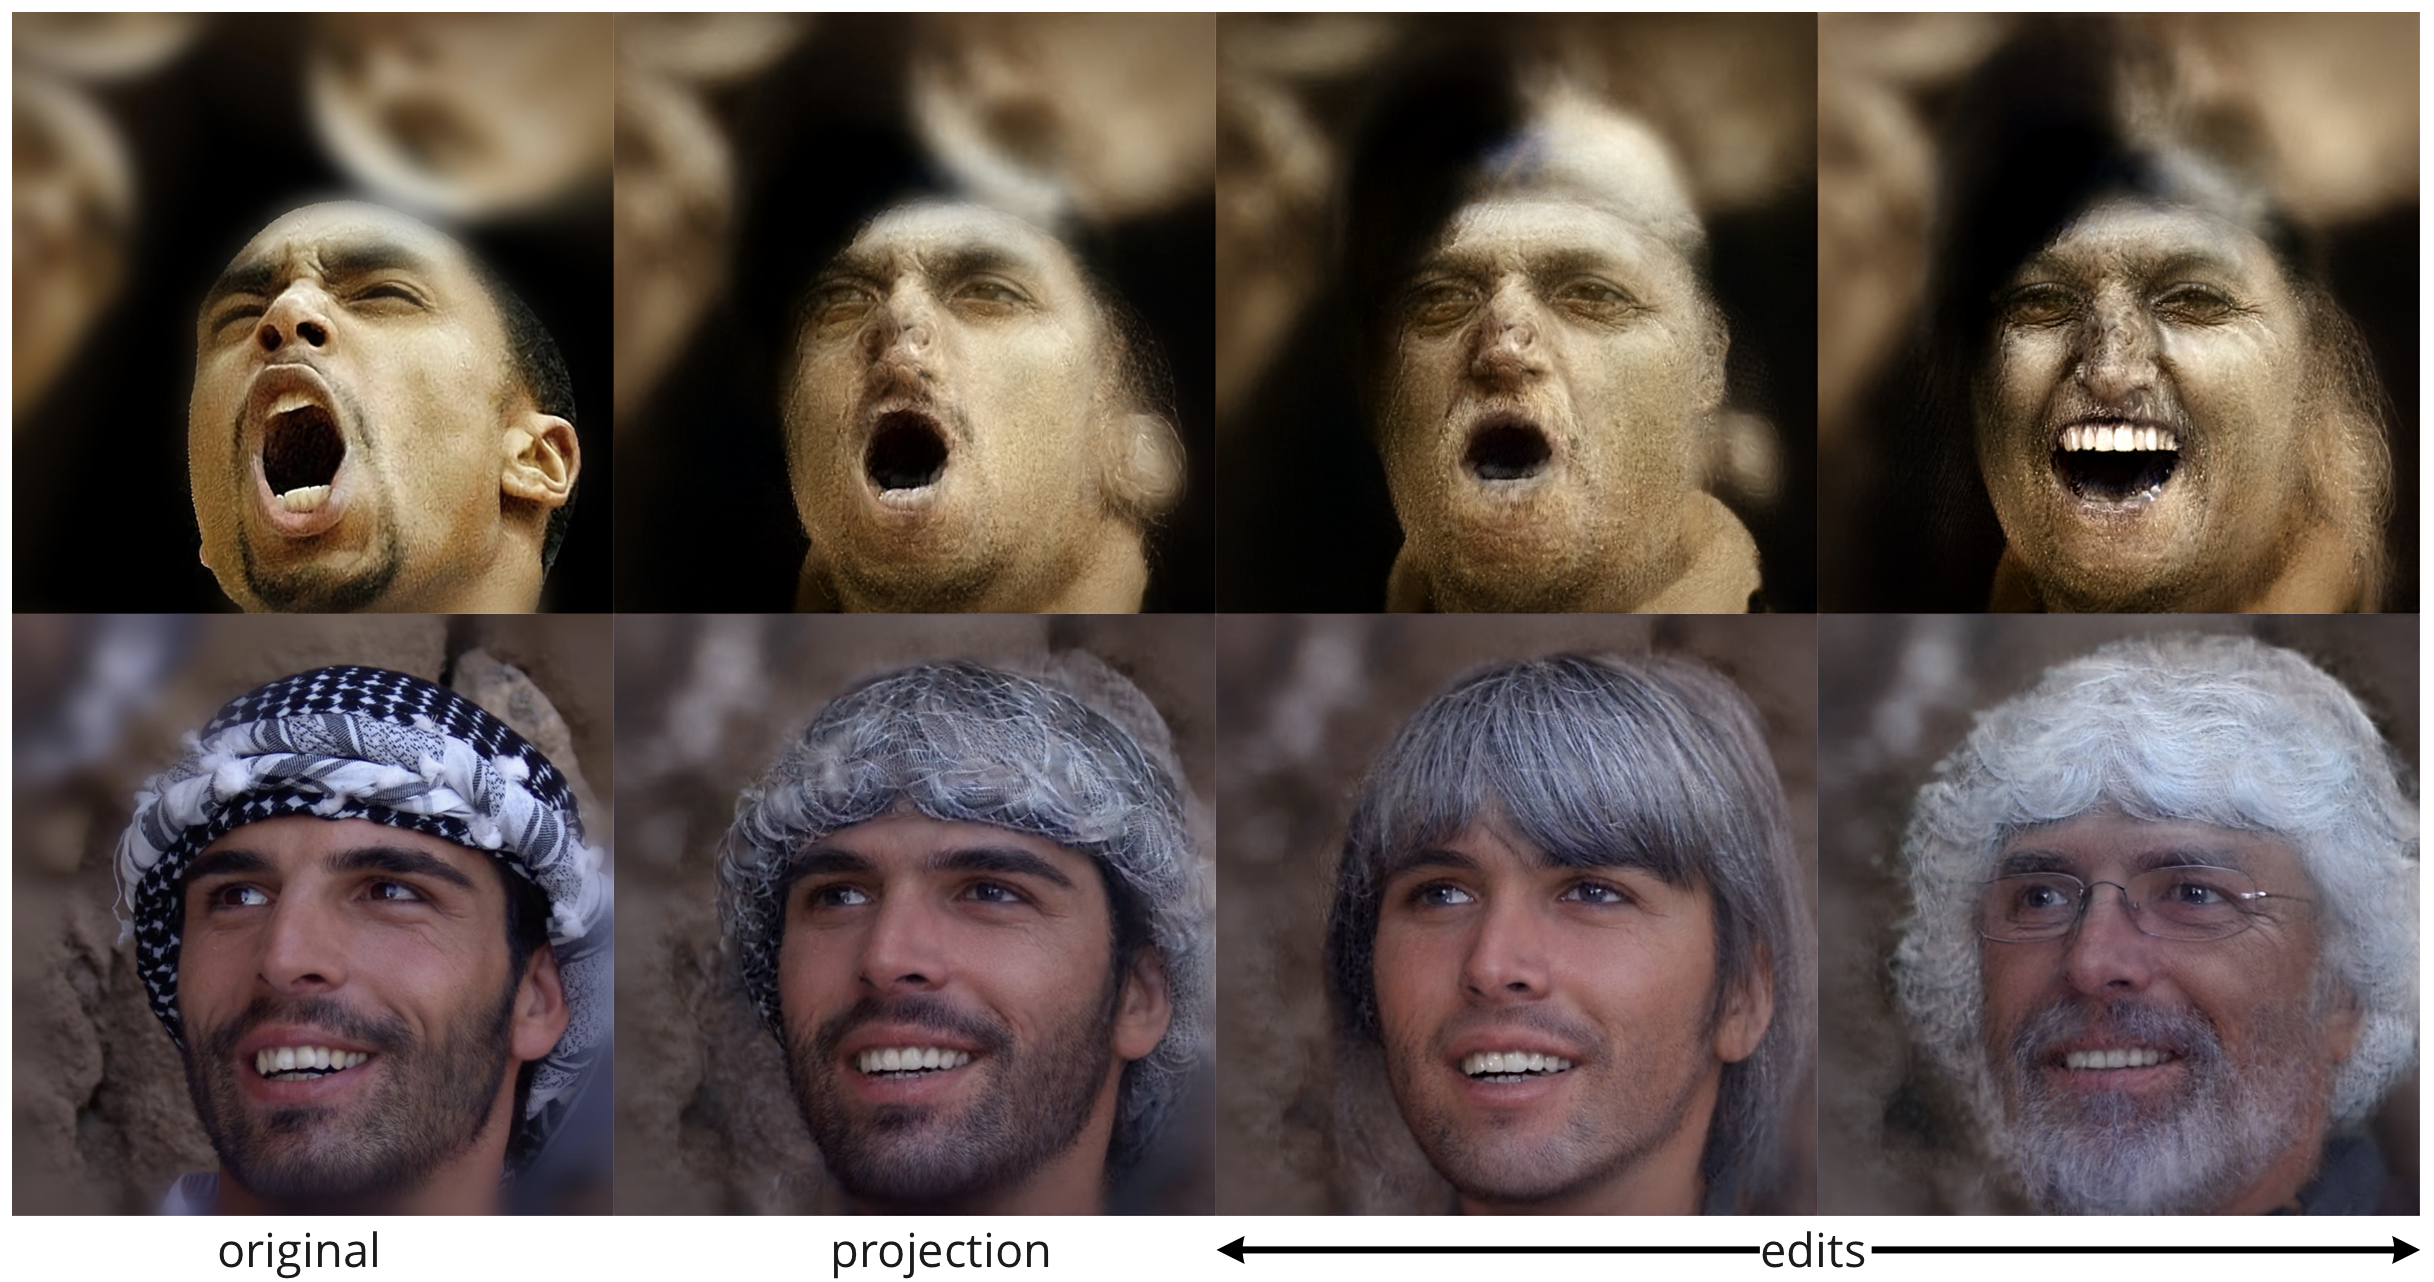
\includegraphics[width=0.75\textwidth]{images/magec/problem_images.png}

\caption{Problematic images for our method. In the first row, an atypical face 
produces a low-quality reconstruction since the image space loss and the latent 
space loss oppose each other: the input image is too out-of-domain. In the
 second row, our method struggles to represent a challenging semantic concept 
 (the keffiyeh). The projection represents the keffiyeh as hair, 
 evidenced by the subsequent edits (\emph{straight hair}, \emph{old age}).}
    \label{fig:problem_images}
\end{figure*}



\section{Conclusion}

We propose a novel GAN-inversion optimization strategy which 
allows supervision on two levels: the image space and the latent
 space. In this way, we are able to integrate editability directly
  in the loss term, resulting in more editable latent vectors when
   applying editing methods. In particular, editing methods not 
   used to supervise the loss perform better than baseline methods,
    suggesting that performing optimization in this way discovers 
    a more ``in-domain'' latent vector. We evaluate qualitatively 
    and quantitatively, and notably introduce a novel 
    \emph{edit consistency score} which specifically evaluates the
     performance of a projection method in terms of editability.
      Our method takes a step forward in performing realistic and 
      high-quality edits on real images.


% In concurrent work, \cite{alaluf2021restyle} proposed an 
% encoder-based method based on \emph{iterative refinement}, in which the latent 
% vector is passed and refined through an encoder multiple times, ressembling 
% the iterative denoising nature of a \ac{DDPM}. They obtained state-of-the-art 
% results for encoder-based methods, and only required 10 forward passes, but their 
% reconstruction still lagged behind optimization-based methods. 
In  concurrent work on optimization-based methods, 
BDInvert \citep{kang2021gan} proposed an inversion method specifically to address the 
poor inversion for out-of-domain translated or rotated images, by extending the 
optimization space to include a feature map in the convolutional \ac{GAN}, which is invariant
to rotation and translation. Finally, later work \citep{feng2022near} achieve 
state-of-the-art optimization-based inversion results, both in terms of editing and reconstruction.
They propose a clever strategy which addresses the limitations posed in section \ref{section:magec_limitations}
by first finding the closest latent $\z$ possible through an encoder-based method 
or optimization-based method, and then optimizing the parameters of the \ac{GAN}
itself to actually change and adapt its manifold to include out-of-domain images 
within its manifold. Because only small tweaking is required to adapt the pre-trained 
\ac{GAN}'s manifold, existing editing methods still work out-of-the-box.

Nevertheless, \ac{GAN} inversion methods are still limited to images from restricted 
domains of a pre-trained \ac{GAN}, largely limiting their use-case to practical settings. 
In the next chapter, we thus try to circumvent inversion completely and examine image 
editing through the lense of optimizing a VQ-GAN \citep{esser2021taming} encoded vector 
before decoding the edited embedding. 

